\section{Experimental setup}

\subsection{Calculating damping ratio}
We will use the logarithmic decrement, $\delta$, to find the damping ratio, $\zeta$:
\begin{align}
    \zeta = \frac{\delta}{ \sqrt{\delta^2 + {(2\pi)}^2} } \text{ where } \delta = \ln\frac{x_{n}}{x_{n+1}} 
\end{align}
\begin{figure}[h]\centering
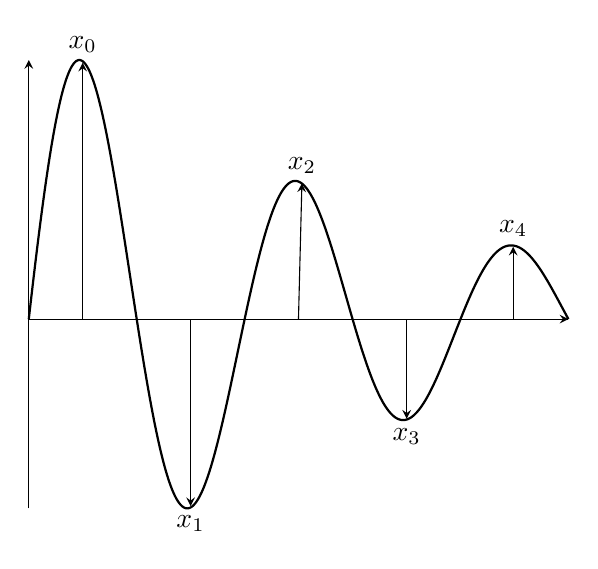
\begin{tikzpicture}
    \def\PItwo{1.5707}
    \begin{axis}[
        domain=0:5*pi, samples=400, smooth,
        xtick=\empty,ytick=\empty,
        axis lines = center, 
        % enlargelimits=true,
        clip=false
        ]
        \addplot[thick] {sin(deg(x))*exp(-0.1*x)};
        \addplot[dashed] {0};
        \draw[-stealth](axis cs: 1.57, 0) -- (axis cs: 1.57,  0.85) node[above]{$x_{0}$};
        \draw[-stealth](axis cs: 4.71, 0) -- (axis cs: 4.71, -0.62) node[below]{$x_{1}$};
        \draw[-stealth](axis cs: 7.85, 0) -- (axis cs: 7.95,  0.45) node[above]{$x_{2}$};
        \draw[-stealth](axis cs: 11.0, 0) -- (axis cs: 11.0, -0.33) node[below]{$x_{3}$};
        \draw[-stealth](axis cs: 14.1, 0) -- (axis cs: 14.1,  0.24) node[above]{$x_{4}$};
    \end{axis}
\end{tikzpicture}
\caption{Visualisation of logarithmic decrement}
\label{fig:visualisation-of-logarithmic-decrement}
\end{figure}